\chapter{Realisierung}
\label{chap:Realisierung}

Dieses Kapitel beschreibt die Realisierung des Prototyps. Der Prototyp ist eine überarbeitete Version der Konzeptvariante 2, siehe Unterkapitel \ref{sec:var2}. Es mussten Änderungen bei verschiedenen Komponenten durchgeführt werden, diese werden im Unterkapitel \ref{sec:mechKomp} erläutert. 

In der Abbildung \ref{fig:realisierung} ist das realisierte Konzept ersichtlich.

\begin{figure}[H]
	\centering
%	\includegraphics[width=0.3\textwidth]{resources/realisierung.PNG}
	\caption[realisiertes Konzept]{realisiertes Konzept}
	\label{fig:realisierung}
\end{figure} 


\section {Hardware}
\label{sec:Hardware}

Da beide Projekte, welche im Unterkapitel \ref{sec:Vorzeigeprojekte} eine endlos drehende Konstruktion nutzen, sowie die Aufgabenstellung im Anhang \ref{Pflichtenheft} eine drehende Konstruktion vorgibt, wurde eine endlos drehende mechanische Konstruktion angefertigt. 

\subsection {mechanische Komponenten \& Gehäuse}
\label{sec:mechKomp}

Um eine möglichst einfache und schnelle Lösung zu realisieren, wurden die mechanischen Komponenten nach Verfügbarkeit ausgewählt. Die Masse des Alurohrs und der Zahnräder waren größtenteils durch die verfügbaren Grösse des Kugellagers gegeben. Das Kugellager wurde so gewählt, dass ein Ethernet RJ45 Stecker hindurchgeführt werden kann, weil der gewählte Schleifring ein vor konfektionierten RJ45-Stecker besitzt. Daraus ergibt sich einen Innendurchmesser von 22 mm und der entsprechende Aussendurchmesser von 44 mm.
Das Kugellager wurde direkt in das Alurohr gepresst und zusätzlich seitlich mit Schrauben verkeilt. Das Alurohr wurde mit Aussendurchmesser 50 mm gewählt und Wandstärke 3mm. Einerseits ist so der Innendurchmesser des Alurohrs passend zum Aussendurchmesser des Kugellagers und anderseits können bei dieser Wandstärke Gewinde geschnitten werden, damit Schrauben als Keil verschraubt werden können..

Der innere Ring des Kugellagers wurde auf den Kugellageradapter gesteckt. Dieser ist wiederum wie in Abbildung \ref{fig:mechKomp} an der Deckplatte befestigt. Somit lässt sich das Alurohr mit wenig Reibung drehen.

Die zwei Zanhräder wurden mit dem CAD-Tool OnShape gelayoutet und im FabLab mit einem 3D-Drucker erzeugt. Das grösse Zahnrad mit 48 Zähnen besitzt den Innendurchmesser 50 mm, welcher dem Alurohr entspricht. Dieses wurde auf das Alurohr gepresst. Das zweite Zahnrad ist im Verhältnis 1.5:1 kleiner und besitzt 32 Zähne. Die Übersetzung wurde so gewählt, dass die Komponenten mit genügend Abstand nebeneinander montiert werden können.  

\begin{figure}[H]
	\centering
	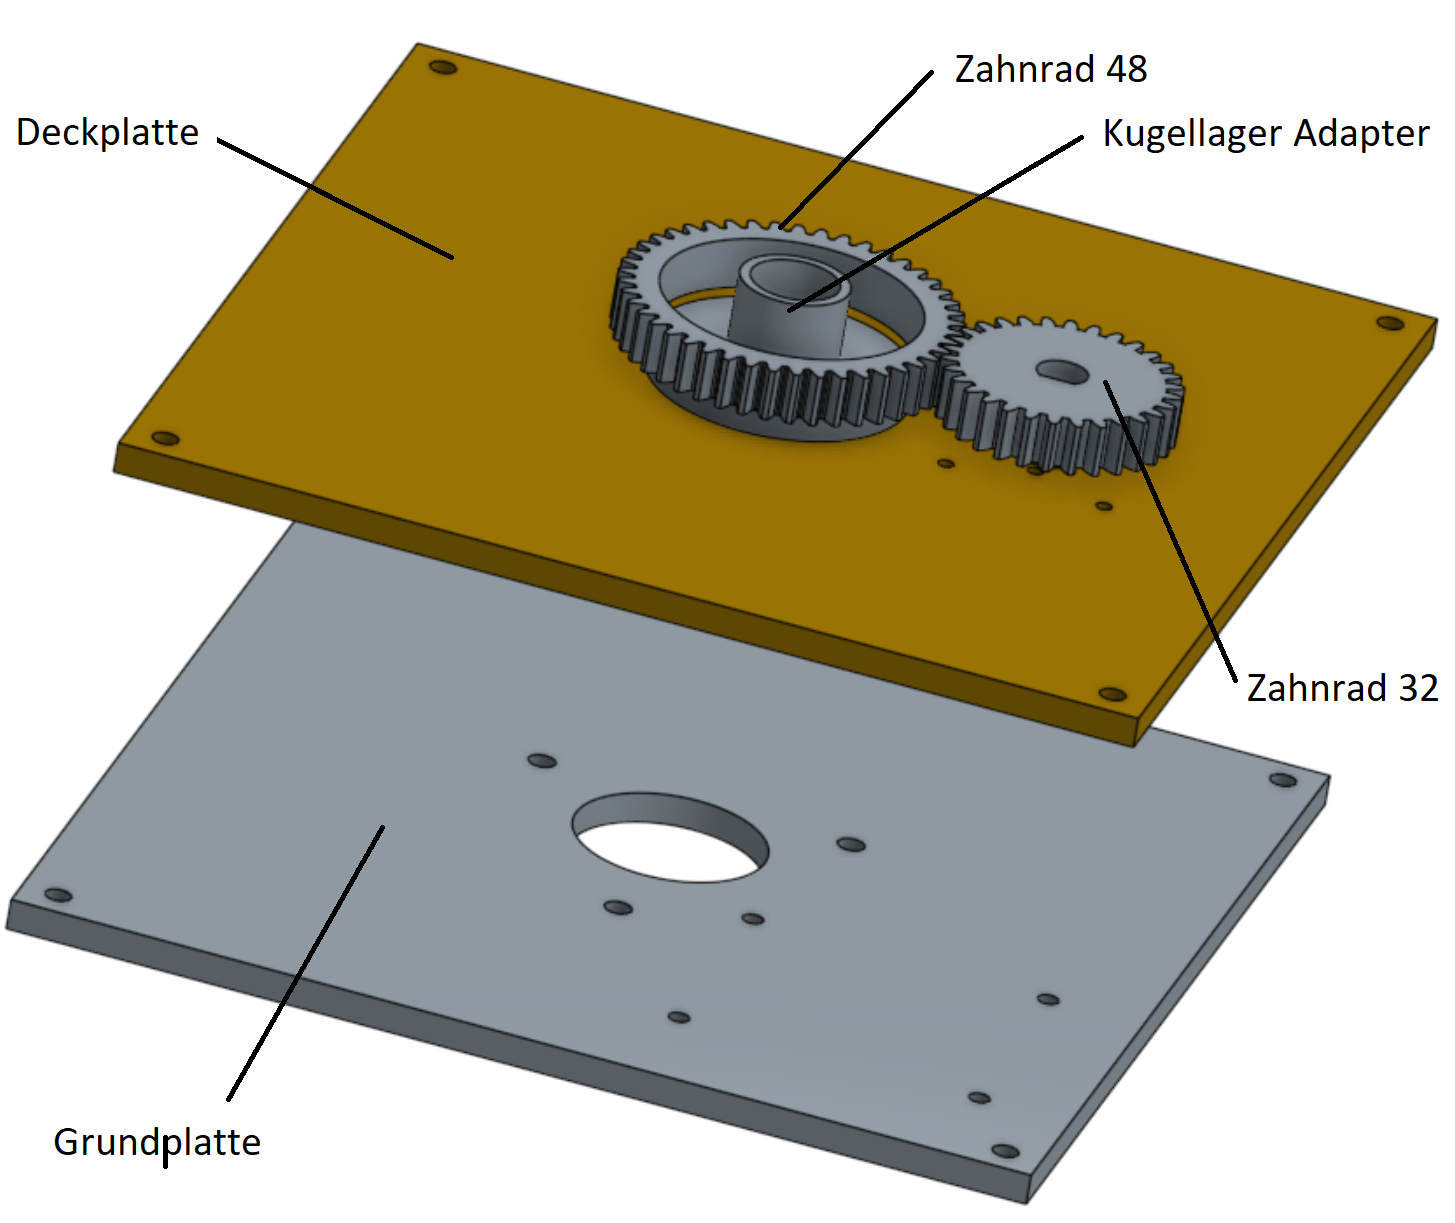
\includegraphics[width=0.8\textwidth]{resources/mechKomp2.PNG}
	\caption{zusammengefügte mechanische Komponenten}
	\label{fig:mechKomp}
\end{figure} 

Die Grösse der Platten wurde so gewählt, dass alle Komponenten dazwischen verbaut werden können. Daher wurden zwei MDF-Platten mit den Massen 200mm x 200mm x 6mm (HxBxT) im Fablab erstellt. Die Grund- und Deckplatten wurden in OnShape gelayoutet und besitzen bereits vorgefertigte Löcher für die Montage der elektrischen Komponenten.


\subsection {elektrische Komponenten}
\label{sec:elekKomp}



% verkabelungsskizze

\section{Software}
\label{sec:SoftwareReal}
Wie bereits im Kapitel Informationsbeschaffung \ref{sec:Software} erläutert wird durch das Velodyne Package ein grosser Teil der Aufgabenstellung bereits abstrahiert. Die einzelnen Aufgabenblöcke wurden nochmals unterteilt und sind in Abbildung \ref{fig:software_flow} dargestellt. Einerseits ist es nötig den Datenstream in einem weiteren Node zu empfangen und anderseits muss die Position ermittelt werden. Diese beiden Daten werden im Node \textit{/velodyne\_combined} zusammengefügt. Sobald die Daten kombiniert werden können, muss in einem weiteren Schritt die kombinierten Daten in einem Container gespeichert werden und bei Bedarf versendet.

\begin{figure}[H]
	\centering
	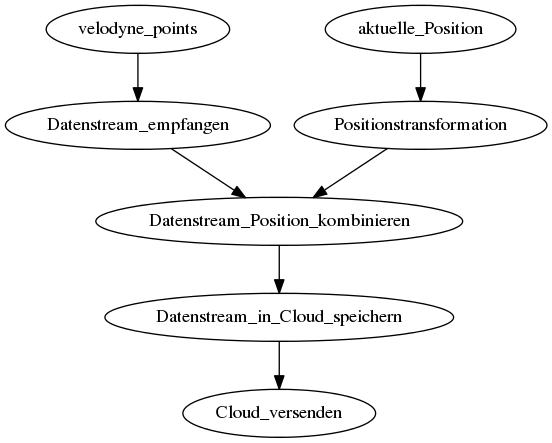
\includegraphics[width=0.5\textwidth]{resources/software_flow.png}
	\caption{Software Ablaufstruktur}
	\label{fig:software_flow}
\end{figure}   

Die Software wurde aufbauend konzipiert. Dabei wurde in einer ersten Phase das Empfangen und Weiterleiten mittels ROS  \textit{Publisher und Subscriber} programmiert. In einem zweiten Schritt wurde die aktuelle Position mit den Daten kombiniert. In der letzte Phase wurde die Software mit dem Zusammenfügen der Datenpunkte erweitert. 

In Abbildung \ref{fig:rqt_graph_erweitert_2} ist mit \textcolor{red}{roter} Umrandung die Softwareerweiterung ersichtlich. Diese wurde in einem eigenen Package namens Laser\_3D erarbeitet. 

\begin{figure}[H]
	\centering
	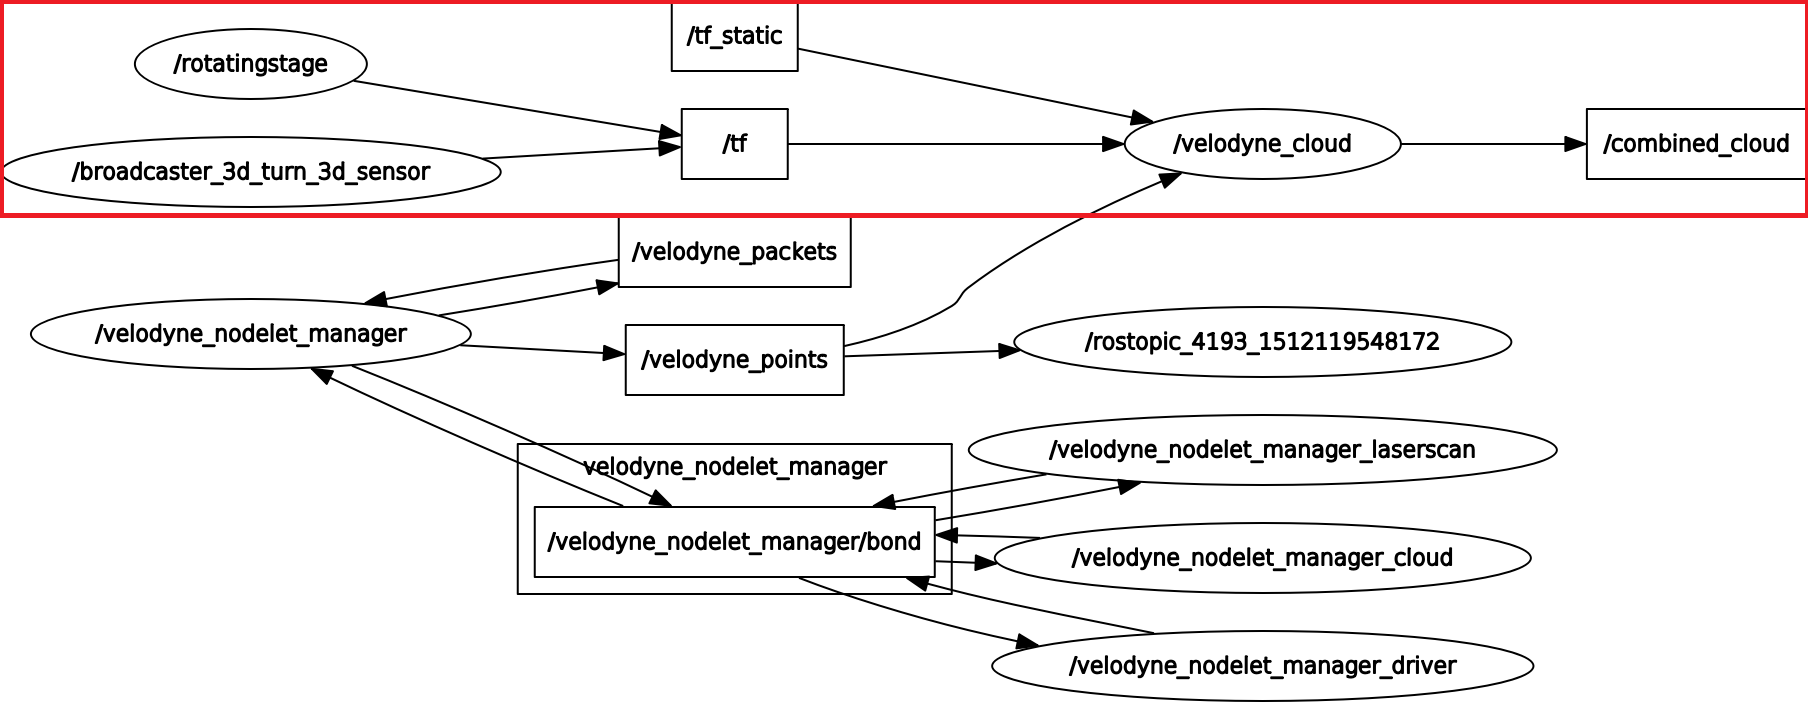
\includegraphics[width=0.8\textwidth]{resources/rqt_graph_erweitert_2.png}
	\caption{zusammengefügte mechanische Komponenten}
	\label{fig:rqt_graph_erweitert_2}
\end{figure} 

\subsection{Phase 1: Empfangen und Weitersenden}

In dieser Phase wurden die Message \textit{velodyne\_points (vom Typ: velodyne\_ msgs/PointCloud2)}

 

\subsection{Phase 2: Kombination Transformation}




\begin{figure}[H]
	\centering
	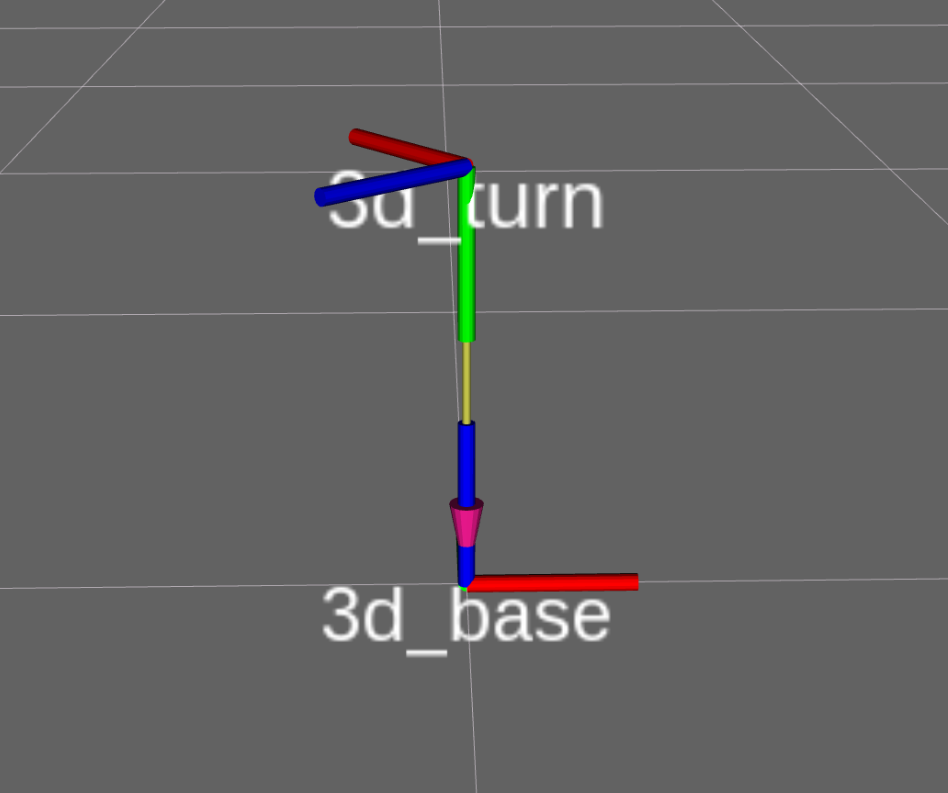
\includegraphics[width=0.5\textwidth]{resources/tf_rotation.PNG}
	\captionV[dynamishce Koordinatentransformation]{dynamische Koordinatentronsformation}
	\label{fig:software_ros}
\end{figure} 



\subsection{Phase 3: Punktwolke erstellen}

\begin{figure}[H]
\centering
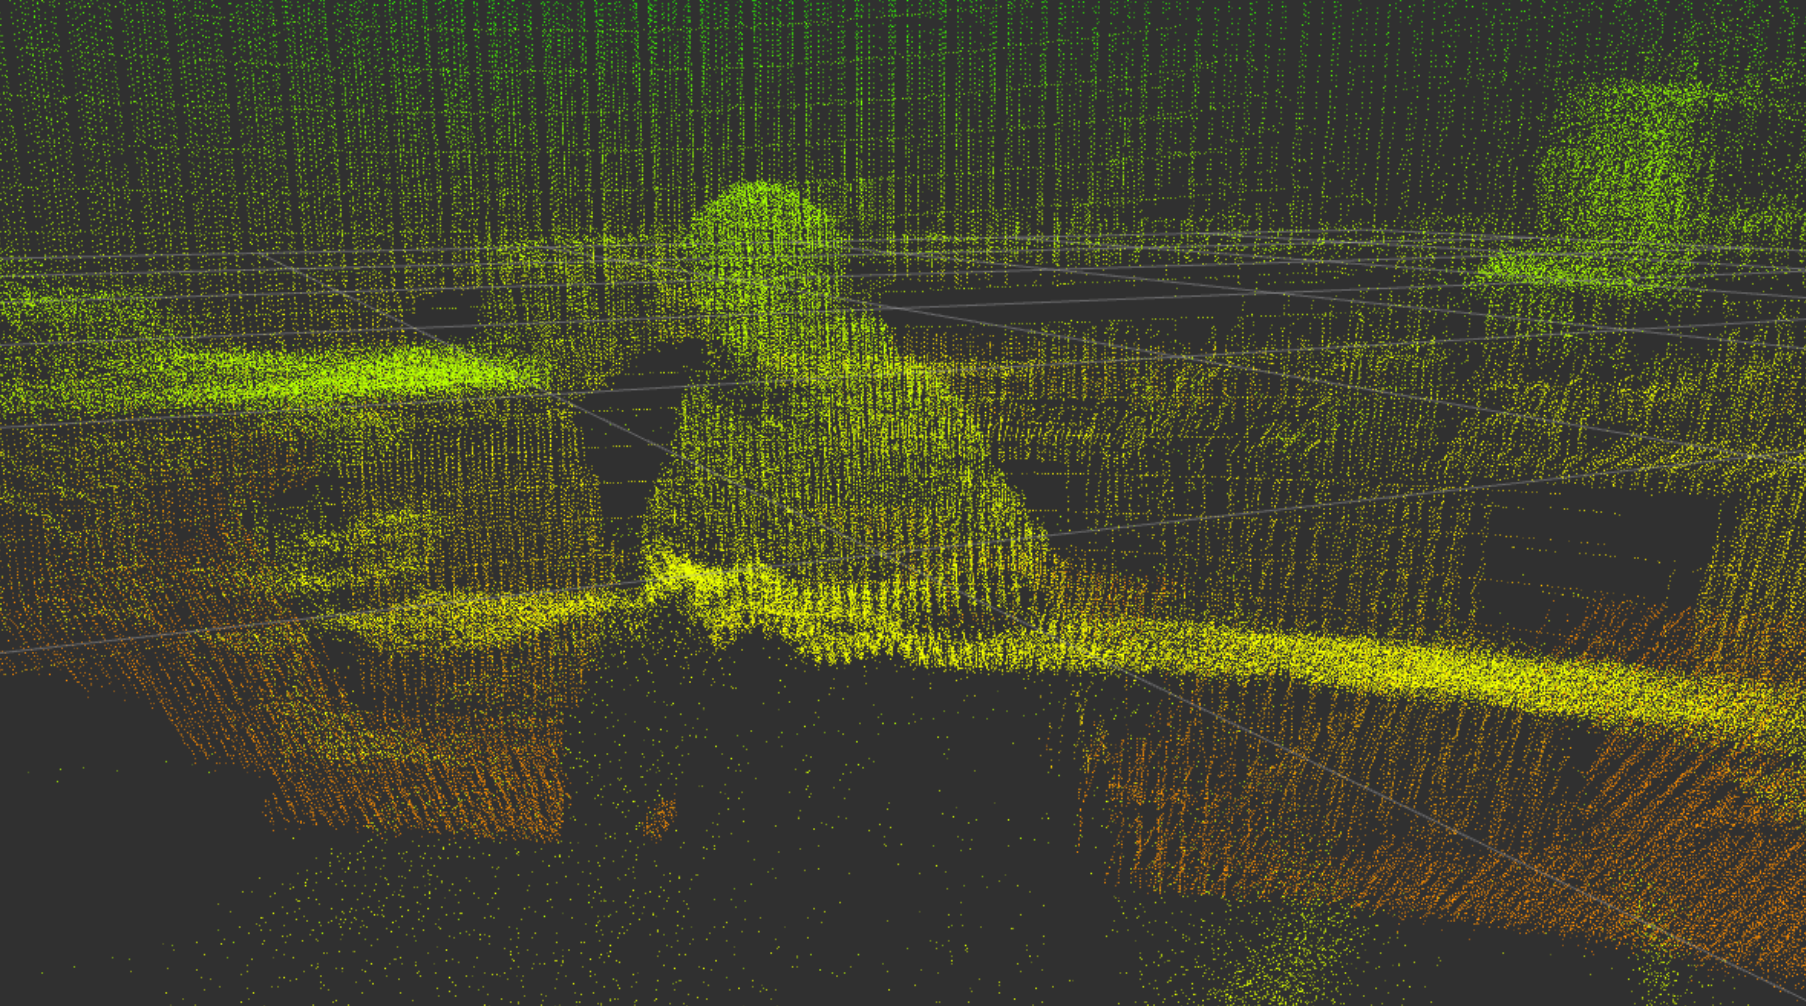
\includegraphics[width=1.0\textwidth]{resources/pointcloud_test.png}
\caption[Punktwolke einer Personbei Distanz 1m]{Punktwolke einer Personbei Distanz 1m}
\label{fig:pointcloud_test}
\end{figure}

\begin{figure}[H]
	\centering
	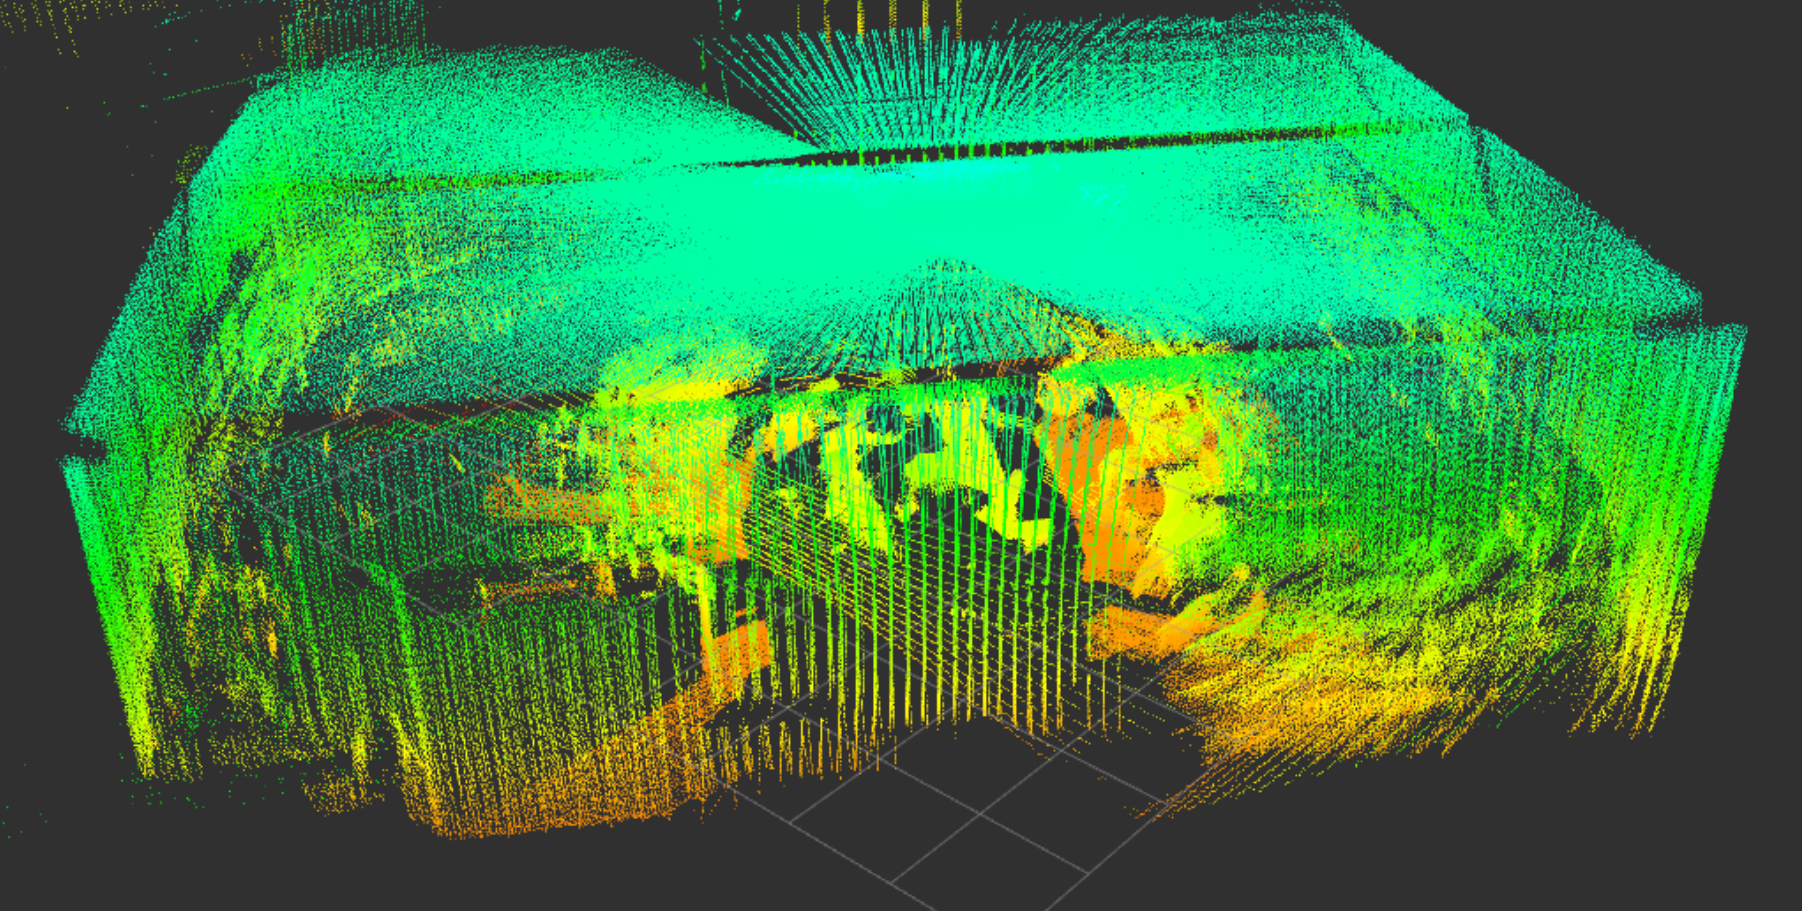
\includegraphics[width=1.0\textwidth]{resources/raumausmessung.png}
	\caption[zusammengefügte Punktwolken]{zusammengefügte Punktwolken}
	\label{fig:raumausmessung}
\end{figure}  


\subsection {Motorenansteuerung}
\label{sec:Motorenansteuerung}

In der Konzeption wurde ein Gleichstrommotor der Marke Pololu für den Antrieb ausgewählt(siehe \ref{subsec:Gleichstrommotor}). Während der Realisierung wurden bedeutende Fehlverhalten des Motors festgestellt. Die angegebenen Encoder Signale entsprechen nicht den zu erwartenden Ergebnissen. Die Messwerte varieren hierbei, um eine umgerechnete Auflösung von 5-10. Dies verursacht unbrauchbare Resultate beim zusammenfügen der Punktwolken.

Der Motor besitzt zusätzlich eine nicht nachvollziehbares Fehlverhalten. In einer Messung des Motorentreibers wurde ein fehlerfreies \ac{PWM} ausgemessen und auch die nötigen Strom (1 Ampere) und Spannungswerte (12 Volt) verifiziert. Dennoch blockiert der Motor willkürlich bei verschiedenen Drehpositionen. Dieses Fehlverhalten könnte auf ein internen Getriebedefekt zurück zu führen zu sein. 

Aus den erwähnten Gründen wurde schnellst möglichst eine Alternative eruiert. Bei der Alternative handelt es sich um einen Schrittmotor der Marke Trinamic. Dieser Motor wurde aus Gründen der Verfügbarkeit und aus bereits bestehenden Kenntnissen ausgewählt. 

Die Software wurde angepasst auf die neue Konfiguration. Nun werden mittels 


\section{Zwischenfazit}
\label{sec:ZwischenfazitReal}
Der 
